\documentclass[main.tex]{subfiles}
\begin{document}
	
	In this section, we present the initial results of our implementation of the GRIN framework. The measurements presented here can only be considered preliminary, given the compiler needs further work to be comparable to systems like the Glasgow Haskell Compiler or the Idris compiler~\cite{idris}. Nevertheless, these statistics are still relevant, since they provide valuable information about the effectiveness of the optimizer.
	
	\subsection{Measured programs}
	
	%TODO: include code of Length
	The measurements were taken using the Idris front end and LLVM back end of the compiler. Each test program --- besides ``Length" --- was taken from the book \textit{Type-driven development with Idris}~\cite{tdd-idris} by Edwin Brady. These are small Idris programs demonstrating a certain aspect of the language.
	
	``Length" is an Idris program, measuring the length of a list containing the natural numbers from 1 to 100. This example was mainly constructed to test how the dead data elimination pass can transform the inner structure of a list into a simple natural number (see Section~\ref{sec:dde}).
	
	\subsection{Measured metrics}
	
	% DONE
	%- idris FR, LLVM BE
	%- small programs from TDD
	%- simple code generation
	%- no GC
	%- pipeline setup
	
	% TODO
	%- cant compare to IC
	%- compile & runtime stats for GRIN IR
	%- runtime stats for binary
	%- optimization levels?
	
	
	\begin{figure}
		\hspace{-0.5cm}
		\renewcommand{\figurename}{Diagram}
		\caption{Length - GRIN statistics}
		\label{diagram:length-stats}
		\addtocounter{figure}{-1}
		\begin{minipage}{0.5\textwidth}
			\subcaption{Runtime}
			\resizebox{\width}{7cm}{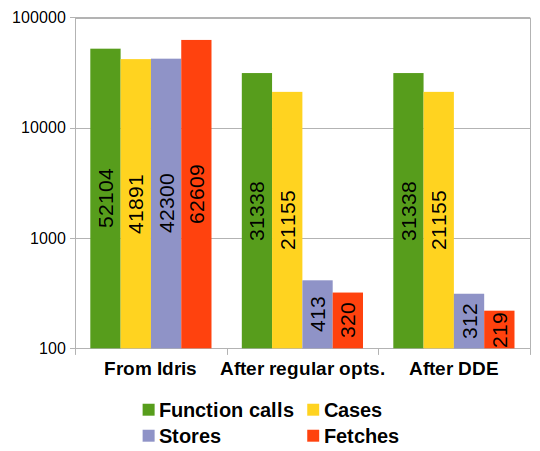
\includegraphics[scale=0.55]{length-runtime.png}}
		\end{minipage}
		\begin{minipage}{0.5\textwidth}
			\subcaption{Compile time}
			\resizebox{\width}{7cm}{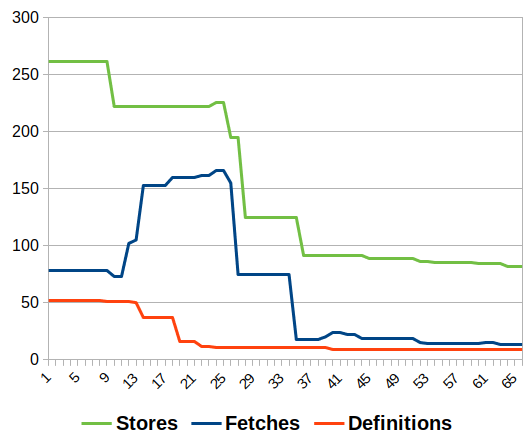
\includegraphics[scale=0.55]{length-compile-time.png}}
		\end{minipage}
	\end{figure}

	\begin{figure}
		\hspace{-0.5cm}
		\renewcommand{\figurename}{Diagram}
		\caption{Exact length - GRIN statistics}
		\label{diagram:exact-length-stats}
		\addtocounter{figure}{-1}
		\begin{minipage}{0.5\textwidth}
			\subcaption{Runtime}
			\resizebox{\width}{7cm}{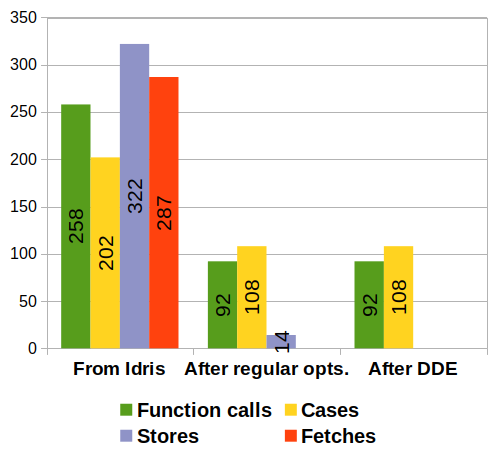
\includegraphics[scale=0.55]{exact-length-runtime.png}}
		\end{minipage}
		\begin{minipage}{0.5\textwidth}
			\subcaption{Compile time}
			\resizebox{\width}{7cm}{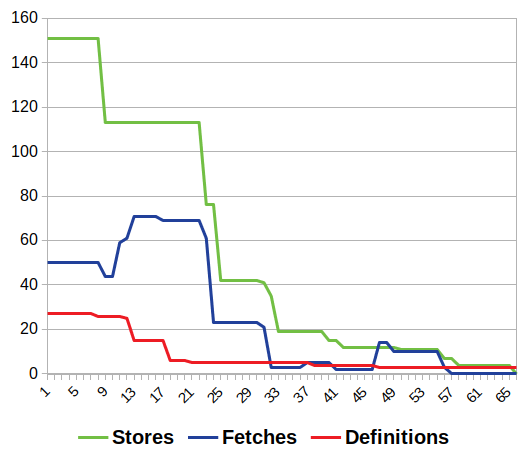
\includegraphics[scale=0.55]{exact-length-compile-time.png}}
		\end{minipage}
	\end{figure}
	
	\begin{figure}
		\hspace{-0.5cm}
		\renewcommand{\figurename}{Diagram}
		\caption{Type level functions - GRIN statistics}
		\label{diagram:tyfuns-stats}
		\addtocounter{figure}{-1}
		\begin{minipage}{0.5\textwidth}
			\subcaption{Runtime}
			\resizebox{\width}{7cm}{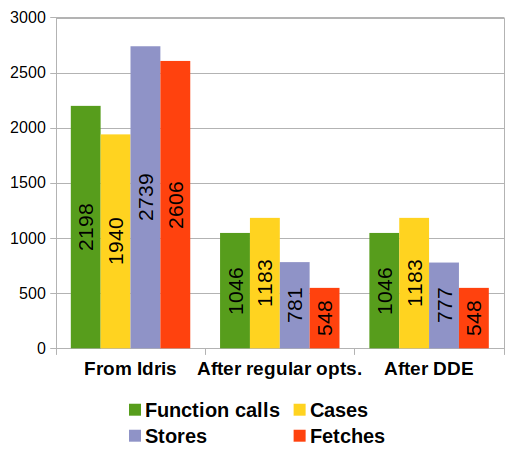
\includegraphics[scale=0.55]{tyfuns-runtime.png}}
		\end{minipage}
		\begin{minipage}{0.5\textwidth}
			\subcaption{Compile time}
			\resizebox{\width}{7cm}{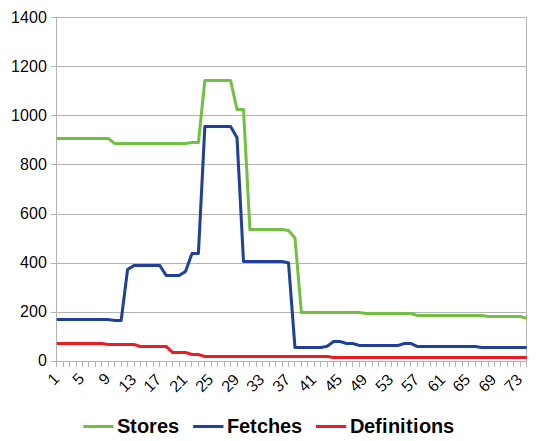
\includegraphics[scale=0.55]{tyfuns-compile-time.png}}
		\end{minipage}
	\end{figure}
	
	\begin{figure}
		\hspace{-0.5cm}
		\renewcommand{\figurename}{Diagram}
		\caption{Reverse - GRIN statistics}
		\label{diagram:reverse-stats}
		\addtocounter{figure}{-1}
		\begin{minipage}{0.5\textwidth}
			\subcaption{Runtime}
			\label{diagram:reverse-stats-a}
			\resizebox{\width}{7cm}{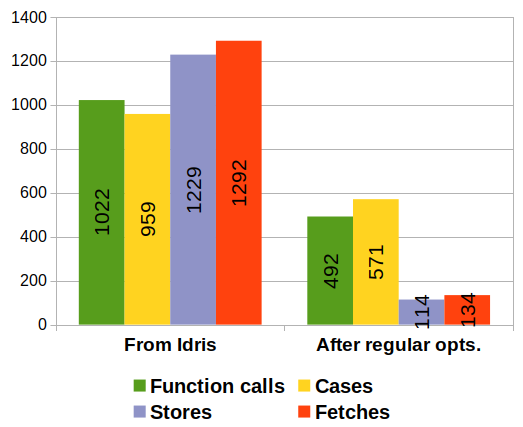
\includegraphics[scale=0.55]{reverse-runtime.png}}
		\end{minipage}
		\begin{minipage}{0.5\textwidth}
			\subcaption{Compile time}
			\label{diagram:reverse-stats-b}
			\resizebox{\width}{7cm}{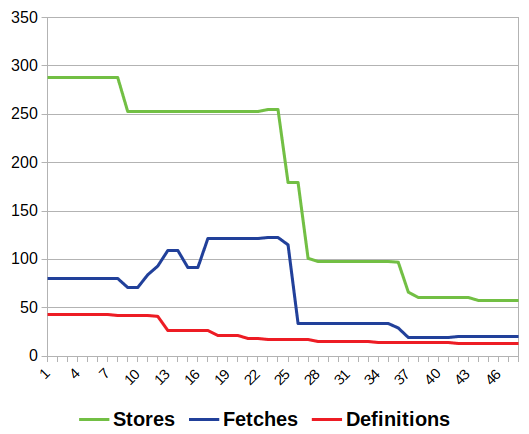
\includegraphics[scale=0.55]{reverse-compile-time.png}}
		\end{minipage}
	\end{figure}
	
	\begin{center}
		\begin{minipage}{0.6\linewidth}
			\captionof{table}{Length - binary statistics}
			\label{table:length-binary-results}
			\begin{tcolorbox}[tab2,tabularx={l||r|r|r|r}]
				Stage                 & Size  & Instructions & Stores & Loads      \\
				\hline\hline
				\pilcode{normal-O0}   & 23928 & 769588 & 212567 & 233305 \\\hline
				\pilcode{normal-O3}   & 23928 & 550065 & 160252 & 170202 \\\hline
				\pilcode{regular-opt} & 19832 & 257397 & 14848  & 45499  \\\hline
				\pilcode{dde-O0}      & 15736 & 256062 & 14243  & 45083  \\\hline
				\pilcode{dde-O3}      & 15736 & 284970 & 33929  & 54555  \\
			\end{tcolorbox}	
		\end{minipage}
	\end{center}
	
	\begin{center}
		\begin{minipage}{0.58\linewidth}
			\captionof{table}{Exact length - binary statistics}
			\label{table:exact-length-binary-results}
			\begin{tcolorbox}[tab2,tabularx={l||r|r|r|r}]
				Stage                 & Size  & Instructions & Stores & Loads      \\
				\hline\hline
				\pilcode{normal-O0}   & 18800 & 188469 & 14852 & 46566 \\\hline
				\pilcode{normal-O3}   & 14704 & 187380 & 14621 & 46233 \\\hline
				\pilcode{regular-opt} & 10608 & 183560 & 13462 & 45214 \\\hline
				\pilcode{dde-O0}      & 10608 & 183413 & 13431 & 45189 \\\hline
				\pilcode{dde-O3}      & 10608 & 183322 & 13430 & 44226 \\
			\end{tcolorbox}	
		\end{minipage}
	\end{center}
	
	\begin{center}
		\begin{minipage}{0.58\linewidth}
			\captionof{table}{Type level functions - binary statistics}
			\label{table:tyfuns-binary-results}
			\begin{tcolorbox}[tab2,tabularx={l||r|r|r|r}]
				Stage                 & Size  & Instructions & Stores & Loads      \\
				\hline\hline
				\pilcode{normal-O0}   & 65128 & 383012 & 49191 & 86754 \\\hline
				\pilcode{normal-O3}   & 69224 & 377165 & 47556 & 84156 \\\hline
				\pilcode{regular-opt} & 36456 & 312122 & 34340 & 71162 \\\hline
				\pilcode{dde-O0}      & 32360 & 312075 & 34331 & 70530 \\\hline
				\pilcode{dde-O3}      & 28264 & 309822 & 33943 & 70386 \\
			\end{tcolorbox}	
		\end{minipage}
	\end{center}
	
	\begin{center}
		\begin{minipage}{0.62\linewidth}
			\captionof{table}{Reverse - binary statistics}
			\label{table:reverse-binary-results}
			\begin{tcolorbox}[tab2,tabularx={l||r|r|r|r}]
				Stage                 & Size  & Instructions & Stores & Loads      \\
				\hline\hline
				\pilcode{normal-O0}      & 27112 & 240983 & 25018 & 58253 \\\hline
				\pilcode{normal-O3}      & 31208 & 236570 & 23808 & 56617 \\\hline
				\pilcode{regular-opt-O0} & 14824 & 222085 & 19757 & 53125 \\\hline
				\pilcode{regular-opt-O3} & 14824 & 220837 & 19599 & 52827 \\
			\end{tcolorbox}	
		\end{minipage}
	\end{center}

\end{document}